%QUESTIONS HERE
%<*mytag1>
\begin{questions}[resume,start=\number\value{questionsi}+1,noitemsep,leftmargin=20mm,labelsep=0.1cm]
\item What does the "-d1" option do? 
\end{questions}
%</mytag1>

%<*mytag2>
\begin{questions}[resume,start=\number\value{questionsi}+1,noitemsep,leftmargin=20mm,labelsep=0.1cm]
\item What is the destination address shown for the Babel packets? What is its significance?
\end{questions}
%</mytag2>

%<*mytag3>
\begin{questions}[resume,start=\number\value{questionsi}+1,noitemsep,leftmargin=20mm,labelsep=0.1cm]
\item What does the "ihu" shown in some of the packets stand for? What does "nh" stand for?
\end{questions}
%</mytag3>

%<*mytag4>
\begin{questions}[resume,start=\number\value{questionsi}+1,noitemsep,leftmargin=20mm,labelsep=0.1cm]
\item Why can't the Ubuntu Desktop ping babel2? (Hint: Wireshark)
\end{questions}
%</mytag4> 

%<*mytag5>
\begin{questions}[resume*,start=\number\value{questionsi}+1,noitemsep,leftmargin=20mm,labelsep=0.1cm]
\item Check Wireshark and find out what's new in the Babel packets.
\end{questions}
%</mytag5> 

%<*mytag6>
\begin{questions}[resume,start=\number\value{questionsi}+1,noitemsep,leftmargin=20mm,labelsep=0.1cm]
\item
\end{questions}
%</mytag6> 

%<*mytag7>
\begin{questions}[resume*,start=\number\value{questionsi}+1,noitemsep,leftmargin=20mm,labelsep=0.1cm]
\item 
\end{questions}
%</mytag7>

%<*mytag8>
\begin{questions}[resume,start=\number\value{questionsi}+1,noitemsep,leftmargin=20mm,labelsep=0.1cm]
\item
\end{questions}
%</mytag8>

%<*mytag9>
\begin{questions}[resume,start=\number\value{questionsi}+1,noitemsep,leftmargin=20mm,labelsep=0.1cm]
\item 
\end{questions}
%</mytag9>

%LISTS HERE

%<*mytag10>
\begin{enumerate}[noitemsep,label=$\circ$,leftmargin=17mm,labelsep=0.5cm]
\item 
\end{enumerate}
%</mytag10>

%<*mytag11>
\begin{enumerate}[noitemsep,label=$\circ$,leftmargin=17mm,labelsep=0.5cm]
\item 
\item
\end{enumerate}
%</mytag11>



%COMMANDS HERE
%<*mytag12>
\begin{enumerate}[noitemsep,leftmargin=10mm,labelsep=0.1cm]
\item [] \textbf{testsecret}
\end{enumerate}
%</mytag12>

%<*mytag13>
\begin{enumerate}[noitemsep,leftmargin=10mm,labelsep=0.1cm]
\item [] \textbf{}
\end{enumerate}
%</mytag13>
%<*mytag14>
\begin{enumerate}[noitemsep,label=$\circ$,leftmargin=17mm,labelsep=0.5cm]
\item [] \textbf{}
\end{enumerate}
%</mytag14>
%<*mytag15>
\begin{enumerate}[noitemsep,leftmargin=10mm,labelsep=0.1cm]
\item [] \textbf{}

\end{enumerate}
%</mytag15>
%<*mytag16>
\begin{enumerate}[noitemsep,leftmargin=10mm,labelsep=0.1cm]
\item [] \textbf{}

\end{enumerate}
%</mytag16>
%<*mytag17>
\begin{enumerate}[noitemsep,leftmargin=10mm,labelsep=0.1cm]
\item [] \textbf{config t}

\end{enumerate}
%</mytag17>
%<*mytag18>
\begin{enumerate}[noitemsep,leftmargin=10mm,labelsep=0.1cm]
\item [] \textbf{config t}
\end{enumerate}
%</mytag18>
%<*mytag19>
\begin{enumerate}[noitemsep,leftmargin=10mm,labelsep=0.1cm]
\item [] \textbf{tail -f /var/log/tac\textunderscore plus.log}
\item [] \textbf{tail -f /var/log/tac\textunderscore plus/tac\textunderscore plus.acct}
\end{enumerate}
%</mytag19>
%<*mytag20>
\begin{enumerate}[noitemsep,leftmargin=10mm,labelsep=0.1cm]
\item [] \textbf{sudo /etc/init.d/tac\textunderscore plus stop}
\item [] \textbf{sudo /etc/init.d/tac\textunderscore plus start}
\end{enumerate}
%</mytag20>
%<*mytag21>
\begin{enumerate}[noitemsep,leftmargin=10mm,labelsep=0.1cm]
\item [] \textbf{telnet 10.10.10.2}
\end{enumerate}
%</mytag21>
%<*mytag22>
\begin{enumerate}[noitemsep,leftmargin=10mm,labelsep=0.1cm]
\item [] \textbf{show run}
\item [] \textbf{show ip in br}
\item [] \textbf{show users}
\end{enumerate}
%</mytag22>
%<*mytag23>
\begin{enumerate}[noitemsep,leftmargin=10mm,labelsep=0.1cm]
\item [] \textbf{hosts}
\end{enumerate}
%</mytag23>
%<*mytag24>
\begin{enumerate}[noitemsep,leftmargin=10mm,labelsep=0.1cm]
\item [] \textbf{services}
\end{enumerate}
%</mytag24>
%<*mytag25>
\begin{enumerate}[noitemsep,leftmargin=10mm,labelsep=0.1cm]
\item [] \textbf{vulns}
\end{enumerate}
%</mytag25>
%<*mytag26>
\begin{enumerate}[noitemsep,leftmargin=10mm,labelsep=0.1cm]
\item [] \textbf{db\_import $<$name of the Nessus scan file including path$>$}
\end{enumerate}
%</mytag26>
%<*mytag27>
\begin{enumerate}[noitemsep,leftmargin=10mm,labelsep=0.1cm]
\item [] \textbf{vulns}
\end{enumerate}
%</mytag27>
%<*mytag28>
\begin{enumerate}[noitemsep,label=$\circ$,leftmargin=14mm,labelsep=0.5cm]
\item
\end{enumerate}
%</mytag28>


%GRAPHICS HERE


%<*mtag1>
\begin{figure}[H]
\centering
\captionsetup{width=.8\linewidth}
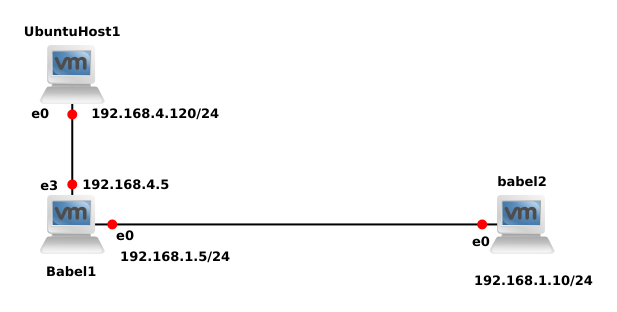
\includegraphics[scale=0.9]{img/Ex1NetDiagram.png}
\caption{Preliminary network topology}
\label{fig:ex1Net}
\centering
\end{figure}
%</mtag1>